%Instruct LaTeX that you would like to format an article and are using a4paper, default is US Letter size!
\documentclass{article}

%Set up a4paper size and sensible margins
\usepackage[a4paper]{geometry}

%Include support for graphics! 
\usepackage{graphicx}
%Include support for url linking
\usepackage{hyperref}

\title{Descriptive title for your report}
\author{ Your full name \& CID }
\date{\today}

\begin{document}

\maketitle


\begin{abstract}
The abstract provides a short summary of the findings contained in the report.  Typically it is one paragraph and starts with one sentence that introduces the work.  Another couple of sentences follow describing the approach taken and quantitative results obtained. 
\end{abstract}

\section{Introduction}
The introduction serves to put the work in context.  You will likely make reference to some background reading here, possibly describing historical background and updating the reader to the most recent knowledge relevant to your report.  Most of the factual statements in the introduction will be derived from external sources and should be referenced.  Some physical principles can be discussed in broad terms in the introduction, but detailed discussion is best left to later sections, if required.   If in doubt, review the guidance provided in the lab manual~\cite{lab_manual}.

\section{Theory}

The theory section outlines the theoretical principles and contains key mathematical formulae are relevant to the report.  Very detailed derivations of results are not required, but important physical steps and assumptions in a derivation can be described and appropriate references given to sources that elaborate the theory in more detail.   
Equations can be inserted into a \LaTeX document either inline by surrounding the expression with \$ symbols, for example $E=mc^{2}$ or as a standalone numbered equation which might be suitable which we express below and reference with an equation number (e.g. the Lorentz transformation shown in equation~\ref{lorentz_transformation}):

\begin{equation}
t' = \gamma \left ( t- \frac{v x}{c^{2}} \right )
\label{lorentz_transformation}
\end{equation}

Using the \textbackslash label{name} command you can give the equation a name which can be referred to later in the document using the \textbackslash ref{name} command, saving you the trouble of having to remember numbers. 

\section{Method}
The method describes the approach you used to obtain the data that you will later present.  It should explain the steps required, materials used and note any special procedures that might not be obvious. It is not a transcript of your lab book!  Ultimately you should describe your procedure in sufficient detail that a competent person at the same level of training as you could repeat your work and verify your results.  When describing how measurements are made, don’t forget to state how accurately you made those measurements.  If it is relevant later in the document to know that voltage was measured to an unusually high level of accuracy, possibly necessitating specialist equipment, then the method is a good place to mention this fact. 
When writing the method, take care to write in the past tense and in the third person, passive voice. Details, such as who did what and your personal opinions are usually not relevant in a scientific document.

You will likely support your writing with a diagram, usually of some apparatus.  A clearly drawn, original diagram is best since you can include all the necessary aspects of the experiment without additional detail.  Avoid the temptation of snapping a quick photograph of the experiment.  This might be useful for the lab book, but in a report, it will convey far too much unnecessary information (e.g. the colour of the bench and presence of lab stools) and not enough about the detail that is important (e.g. the output impedance of an instrument).   Likewise, scanning a diagram from the lab manual or pasting something vaguely relevant from the internet is unlikely to be the best way of communicating the scientifically important aspects of the experiment. 
 
There are a number of programs that can be used to draw diagrams, including some free open source packages such as Dia 
(see 
\url{http://en.wikipedia.org/wiki/List_of_vector_graphics_editors}).  
The ICT software shop offers substantial discounts on professional line-art software such as Corel Draw and Adobe Illustrator available at a discount.  With most of these pieces of software, it will take an hour or two of practice to become proficient. Many of the diagrams in the 1Y lab manual have been drawn using Adobe Illustrator, an example is shown in Figure~\ref{illustrator_example}.

It is permissible to draw diagrams on paper and scan them into the document, or even leave a space in the report and draw the diagram directly onto the report, or glue in a suitable figure.  The paper copy submitted must have the diagrams present, the electronic version submitted can have photos of the artwork inserted.  The underlying principle is clarity, so avoid scrappy sketches but take care to make your diagrams clear and tidy.

Ensure that all diagrams and figures are numbered and have captions.  \LaTeX helps you with this, automatically numbering figures and allowing labels and captions to be associated with figures directly.  You can reference figures using the \\ref command, as for equations.  Note that \LaTeX will try to place your figures where it thinks they will fit best.  If you do not like where \LaTeX is placing your figures, you can force it to put them in a specific place in the document using the [h] option, e.g. \textbackslash begin\{figure\}[h].

\begin{figure}
\centering
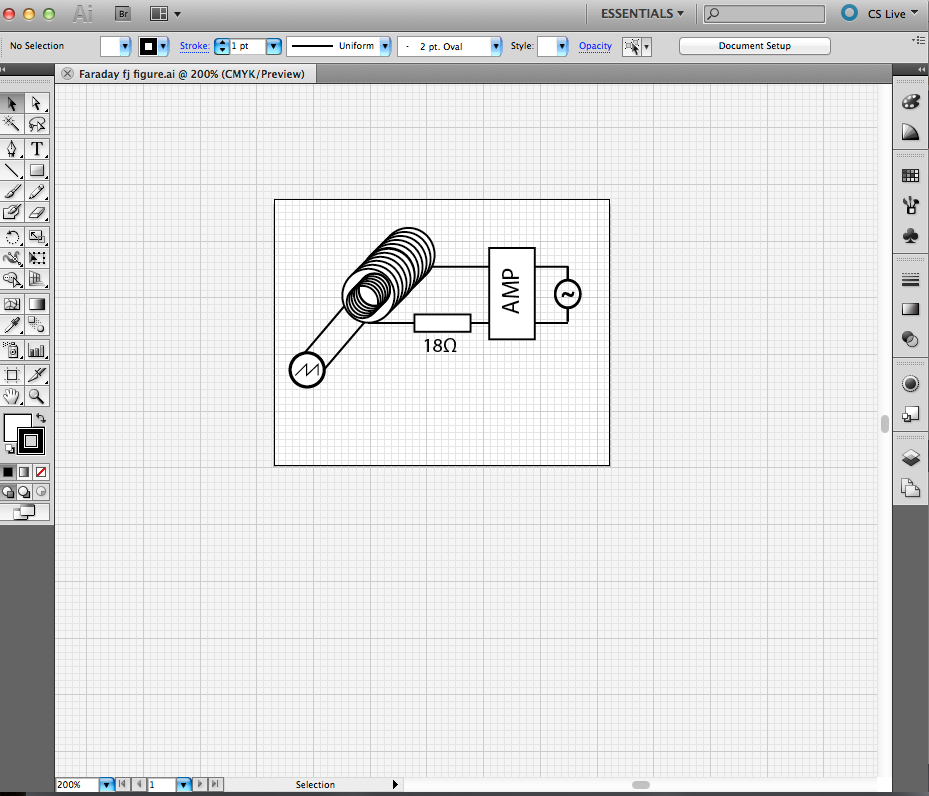
\includegraphics[width=10cm]{example_figure.png}
\caption{Example of a figure being drawn using Adobe Illustrator}
	\label{illustrator_example}
\end{figure}

\section{Results}
The Results section should present the results required to support the finding of your report.  Often these will be presented in a graph or table.  There is no need to present both, if the data has been plotted effectively, the data can remain in your lab-book.   
Consider the uncertainties in your data and if this involved propagating uncertainties, explain how you handled the uncertainties.  It is usually not necessary to restate the standard uncertainty formulae that are present in the lab manual.  Rather these can be referred to in a statement clarifying what was done.   Where uncertainty analysis goes beyond simple addition, products and quotients, then it may justified to add some additional detail, possibly in an appendix if the treatment is particularly involved and risks distracting the reader from the main flow of results.  Whenever possible, datapoints on graphs should be plotted with error bars.
Your results will not be meaningful on their own, so some discussion of their validity and comparison with other known or accepted data will be necessary.  The discussion should be as objective as possible and be based on the measured data.  There will be aspects of the results that could be improved in the future, so you should give the reader a few pointers to areas where improvements would be beneficial and outline what, in your opinion, those improvements might be.

\section{Conclusion}
Restate the aims and findings of the work reported.  The discussion should be brought to a meaningful end here, but take care not to introduce substantially new material into the conclusion.  It should be a tidy series of statements on the findings of the work reported and some of the potential improvements to the work in the future. 

\section{Bibliography}
The reference list is a list of numbered references to supporting documents that you refer to in the text; see for example your lab-manual~\cite{lab_manual}, your 1Y textbook~\cite{young_freedman}, a landmark nanophotonics paper~\cite{ebbesen:98} and finally the 2013 Nobel prize~\cite{nobel_prize}.  It is preferable to cite physical documents that are properly archived, such as books or research papers.  Web-links are quick and easy, but the content will change over time (e.g. Wikipedia pages) so if you do cite a URL, it should be accompanied with a date when the information is valid and suitable title. Some examples are given below:

\begin{thebibliography}{1}
\bibitem {lab_manual} 1st year lab manual 2013-14, Imperial College London.
\bibitem {young_freedman} University Physics, Young and Freedman, 11th Edition, Academic Press, 2006
\bibitem {ebbesen:98} T. W. Ebbesen, H. J. Lezec, H. F. Ghaemi, T. Thio, and P. A. Wolff, “Extraordinary optical transmission through sub-wavelength hole arrays,” Nature, vol. 391, no. 6668, pp. 667–669,  1998. 
\bibitem {nobel_prize} “Peter Higgs and François Englert win Nobel Prize in Physics”, blog maintained by Alok Jha,  Guardian web-page accessed 11/11/2013 \url{http://www.theguardian.com/science/2013/oct/08/nobel-prize-in-physics-live-blog}
\end{thebibliography}

As with figures and equations, each entry into the reference list can be given a label that is then referred to using the \textbackslash cite{} command.  Note this is different to the \textbackslash ref{} command that is used for figures and equations.  You will need to run \LaTeX at least twice to get the numbering of your references and figures correct.

\section{Appendices (optional)}
An appendix is an optional section for when you would like to include additional detail, for example, the derivation of theoretical results, a listing of a computer program or other bulky item that would break up the flow of the report.  In this case you can put an appendix including this detail at the end of the report and refer to it in the text. Do not put important graphs of results in an appendix. Your data are of prime importance and should appear in the main body of the text. 





\end{document}
